\documentclass[aspectratio=169,11pt]{beamer}

\usetheme{default}
\usecolortheme{default}
\setbeamertemplate{navigation symbols}{}

\definecolor{gdpPurple}{HTML}{633E88}
\definecolor{gdpDarkBlue}{HTML}{0C406D}
\definecolor{gdpNavy}{HTML}{091932}
\definecolor{gdpOrange}{HTML}{DD7A0F}
\definecolor{gdpSlate}{HTML}{3B4950}
\definecolor{gdpLightGray}{HTML}{E7E6E6}
\definecolor{gdpBurgundy}{HTML}{820E21}

\setbeamercolor{background canvas}{bg=white}
\setbeamercolor{normal text}{fg=gdpSlate}
\setbeamercolor{frametitle}{fg=gdpPurple,bg=white}
\setbeamercolor{framesubtitle}{fg=gdpDarkBlue,bg=white}
\setbeamercolor{title}{fg=gdpPurple}
\setbeamercolor{subtitle}{fg=gdpDarkBlue}
\setbeamercolor{author}{fg=gdpSlate}
\setbeamercolor{institute}{fg=gdpSlate}
\setbeamercolor{date}{fg=gdpSlate}
\setbeamercolor{item}{fg=gdpDarkBlue}
\setbeamercolor{subitem}{fg=gdpPurple}
\setbeamercolor{block title}{fg=white,bg=gdpDarkBlue}
\setbeamercolor{block body}{fg=gdpSlate,bg=gdpLightGray!30}
\setbeamercolor{block title alerted}{fg=white,bg=gdpBurgundy}
\setbeamercolor{block body alerted}{fg=gdpSlate,bg=gdpLightGray!30}
\setbeamercolor{footline}{fg=gdpSlate}

\usepackage{helvet}
\renewcommand{\familydefault}{\sfdefault}
\usepackage{amsmath,amssymb,graphicx,booktabs,array,xcolor, colortbl}
\usepackage{pifont}
\newcommand{\cmark}{\ding{51}}
\newcommand{\xmark}{\ding{55}}

\setlength{\tabcolsep}{3pt}
\setbeamertemplate{itemize/enumerate body begin}{\small}
\setbeamertemplate{itemize/enumerate subbody begin}{\footnotesize}
\addtolength{\leftmargini}{-0.3cm}
\addtolength{\leftmarginii}{-0.2cm}

\setbeamertemplate{frametitle}{%
  \vspace{0.2cm}
  \textbf{\large\insertframetitle}
  \vspace{0.05cm}
  \par\textcolor{gdpDarkBlue}{\rule{\textwidth}{1.2pt}}
  \vspace{-0.3cm}
}

\setbeamertemplate{footline}{%
  \leavevmode%
  \hbox{%
    \begin{beamercolorbox}[wd=.333\paperwidth,ht=2.5ex,dp=1ex,leftskip=0.3cm]{footline}%
      \insertshortauthor
    \end{beamercolorbox}%
    \begin{beamercolorbox}[wd=.333\paperwidth,ht=2.5ex,dp=1ex,center]{footline}%
      \insertshorttitle
    \end{beamercolorbox}%
    \begin{beamercolorbox}[wd=.333\paperwidth,ht=2.5ex,dp=1ex,rightskip=0.3cm]{footline}%
      \insertframenumber{}
    \end{beamercolorbox}%
  }%
}

\setbeamertemplate{title page}{
  \vspace{1.5cm}
  \begin{center}
    {\Huge\bfseries\textcolor{gdpPurple}{\inserttitle}}\\[0.4cm]
    {\Large\textcolor{gdpDarkBlue}{\insertsubtitle}}\\[1.2cm]
    {\large\textcolor{gdpSlate}{\insertauthor}}\\[0.3cm]
    {\normalsize\textcolor{gdpSlate}{\insertinstitute}}\\[0.3cm]
    {\normalsize\textcolor{gdpSlate}{\insertdate}}
  \end{center}
}

\title{Fluid Neural Networks}
\subtitle{Progress Review — 9 June 2026}
\author{MSc Individual Research Project}
\institute{Cranfield University\hspace{0.3cm}|\hspace{0.3cm}Supervisors: Prof. Weisi Guo, Prof. Takis Tsoutsanis}
\date{9 June 2026}

\begin{document}

% ============================================================
\begin{frame}[plain]
  \titlepage
\end{frame}

% ============================================================
\begin{frame}{Where We Started}
  \textbf{Thermoviscous tuning: local heating $\rightarrow$ viscosity gradient $\rightarrow$ trainable weight}

  \vspace{0.5cm}
  \begin{columns}[T]
    \begin{column}{0.48\textwidth}
      \begin{block}{\footnotesize What we tested}
        \footnotesize
        \begin{itemize}
          \item 12 heat patterns
          \item Re = 10--100
          \item Readout: 2 Hz / 3 Hz amplitude ratio
        \end{itemize}
      \end{block}
    \end{column}
    \begin{column}{0.48\textwidth}
      \begin{alertblock}{\footnotesize What we found}
        \footnotesize
        Ratio = 1.710974046 across \textbf{all} configurations.\\
        Invariant to machine precision.\\
        Advection homogenises temperature.
      \end{alertblock}
    \end{column}
  \end{columns}

  \vspace{0.5cm}
  \begin{center}
    \textcolor{gdpBurgundy}{\large Rigorously tested and eliminated.}
  \end{center}
\end{frame}

% ============================================================
\begin{frame}{The Pivot}
  \textbf{If temperature doesn't work, what does?}

  \vspace{0.5cm}
  \begin{columns}[T]
    \begin{column}{0.48\textwidth}
      \begin{block}{\footnotesize New direction}
        \footnotesize
        Obstacle-mediated wake routing.\\
        Geometry = weights.\\
        Flow = computation.
      \end{block}
    \end{column}
    \begin{column}{0.48\textwidth}
      \begin{block}{\footnotesize Solver}
        \footnotesize
        Face-consistent collocated projection.\\
        Modular obstacle models.\\
        Validated against theory.
      \end{block}
    \end{column}
  \end{columns}
\end{frame}

% ============================================================
\begin{frame}{The Setup}
  \textbf{Geometry, BCs, and solver.}

  \vspace{0.3cm}
  \begin{columns}[T]
    \begin{column}{0.48\textwidth}
      \footnotesize
      \textbf{Domain:}\\
      $5\,\text{mm} \times 2.5\,\text{mm}$\\
      $100 \times 50$ cells ($\Delta x = 50\,\mu\text{m}$)

      \vspace{0.3cm}
      \textbf{Boundary conditions:}\\
      Inlet: parabolic profile, ramped 0--1 s\\
      Outlet: zero-gradient\\
      Walls: no-slip

      \vspace{0.3cm}
      \textbf{Initial condition:}\\
      $\mathbf{u} = 0$, $p = 0$
    \end{column}
    \begin{column}{0.48\textwidth}
      \footnotesize
      \textbf{Solver:}\\
      Incompressible NS, 2D

      \vspace{0.3cm}
      \textbf{Obstacle models:}\\
      Hard-wall mask (squares)\\
      Brinkman alpha (circles / porous)
    \end{column}
  \end{columns}
\end{frame}

% ============================================================
\begin{frame}{What We Found}
  \textbf{Three results that matter.}

  \vspace{0.4cm}
  \footnotesize
  \begin{table}
    \centering
    \renewcommand{\arraystretch}{1.2}
    \begin{tabular}{@{}p{3.5cm}p{4cm}p{5cm}@{}}
      \toprule
      \textbf{Result} & \textbf{What} & \textbf{Why it matters} \\
      \midrule
      Vortex shedding & Circular cylinder at Re = 500 sheds at 10.5 Hz & Nonlinear dynamics exist \\
      Lock-in & Wake synchronises to inlet forcing (8--14 Hz) & System is responsive \\
      \rowcolor{gdpLightGray!50}
      \textbf{XOR gate} & \textbf{Single cylinder + two probes = XOR} & \textbf{Natural computation} \\
      \bottomrule
    \end{tabular}
  \end{table}
\end{frame}

% ============================================================
\begin{frame}{The Headline Result}
  \textbf{A single circular cylinder computes XOR.}

  \vspace{0.3cm}
  \begin{columns}[T]
    \begin{column}{0.38\textwidth}
      \footnotesize
      \textbf{Setup:}
      \begin{itemize}
        \item Two inlet strips
        \item Two probes downstream
        \item Output = $u_{\text{top}} - u_{\text{bottom}}$
      \end{itemize}

      \vspace{0.3cm}
      \textbf{Truth table:}
      \begin{itemize}
        \item (0,0): 0
        \item (1,0): 0.028
        \item (0,1): 0.030
        \item (1,1): 0.002
      \end{itemize}
    \end{column}
    \begin{column}{0.58\textwidth}
      \begin{center}
        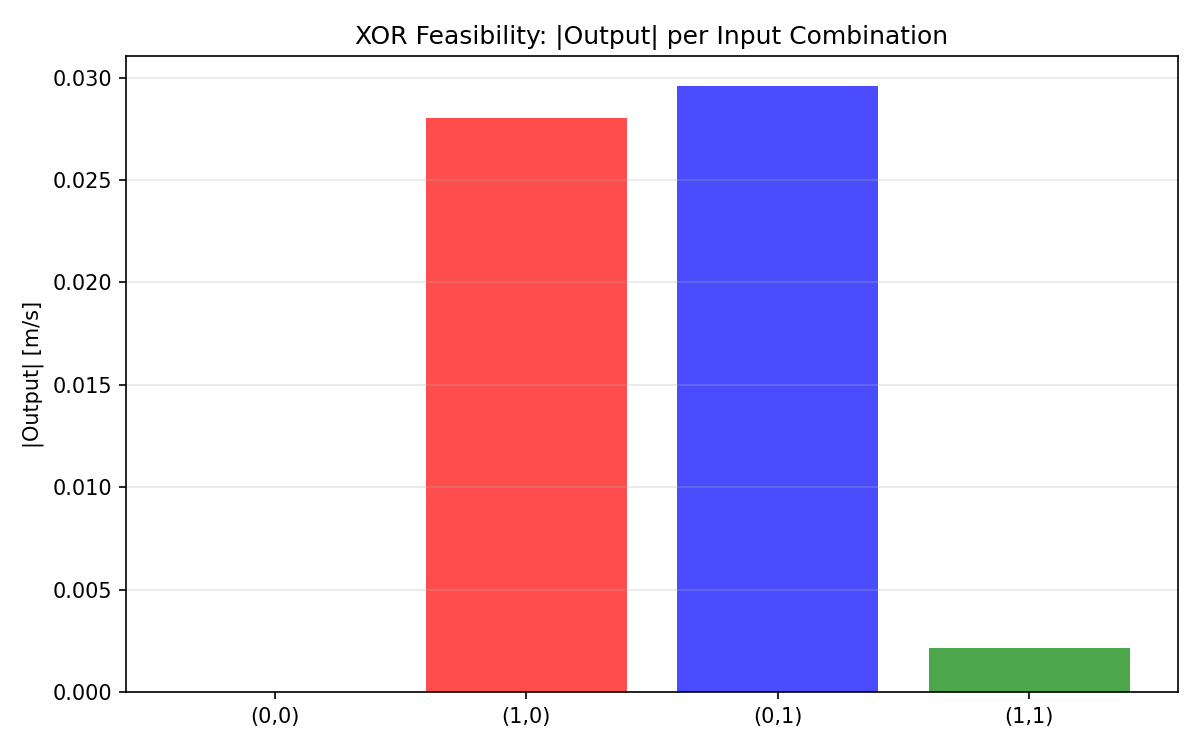
\includegraphics[width=0.95\textwidth]{xor_two_probe_bars.png}
      \end{center}
    \end{column}
  \end{columns}
\end{frame}

% ============================================================
\begin{frame}{How It Works}
  \textbf{The cylinder wake routes flow like a switch.}

  \vspace{0.3cm}
  \begin{columns}[T]
    \begin{column}{0.32\textwidth}
      \begin{center}
        \textbf{(1,0)}\\
        \footnotesize
        Asymmetric wake\\
        deflects \textbf{up}\\
        \vspace{0.2cm}
        Output = +0.028
      \end{center}
    \end{column}
    \begin{column}{0.32\textwidth}
      \begin{center}
        \textbf{(0,1)}\\
        \footnotesize
        Asymmetric wake\\
        deflects \textbf{down}\\
        \vspace{0.2cm}
        Output = $-$0.030
      \end{center}
    \end{column}
    \begin{column}{0.32\textwidth}
      \begin{center}
        \textbf{(1,1)}\\
        \footnotesize
        Symmetric wake\\
        both probes equal\\
        \vspace{0.2cm}
        Output $\approx$ 0
      \end{center}
    \end{column}
  \end{columns}

  \vspace{0.5cm}
  \begin{center}
    \textcolor{gdpDarkBlue}{\large Single input $\rightarrow$ large $|\text{output}|$. Both inputs $\rightarrow$ cancellation.}
  \end{center}
\end{frame}

% ============================================================
\begin{frame}{The Fork in the Road}
  \textbf{Two possible directions. I need guidance on which to pursue.}

  \vspace{0.5cm}
  \begin{columns}[T]
    \begin{column}{0.48\textwidth}
      \begin{block}{\footnotesize Direction A: Frequency domain}
        \footnotesize
        Two-frequency inlet mixing.\\
        NS nonlinearity creates sum/difference.\\
        Signal processing perspective.
      \end{block}
    \end{column}
    \begin{column}{0.48\textwidth}
      \begin{block}{\footnotesize Direction B: Trainable alpha}
        \footnotesize
        Optimise obstacle shape for XOR/AND/OR.\\
        Parameterised Gaussian blobs.\\
        Neural network perspective.
      \end{block}
    \end{column}
  \end{columns}

  \vspace{0.5cm}
  \begin{center}
    \textcolor{gdpBurgundy}{\large Or both?}
  \end{center}
\end{frame}

% ============================================================
\begin{frame}{What I Need From You}
  \begin{enumerate}
    \item \textbf{Scope:} Is XOR sufficient, or do I need multi-bit / trainable weights?
    \item \textbf{Direction:} Frequency mixing or spatial obstacle optimisation?
    \item \textbf{Validation:} OpenFOAM essential or nice-to-have?
    \item \textbf{Timeline:} What's realistic to complete by September?
  \end{enumerate}
\end{frame}

\end{document}
